\documentclass{article}
\usepackage{../mathclub}

\title{Game Theory}
\author{UCSB}
\date{October 17, 2022}

\begin{document}


\section{Introduction}
Welcome to the Week 4 Math Club meeting!
(\emph{Week 4?} yep. crazy.)
This week's handout is all about \emph{game theory}.
Section 1 contains a basic introduction to game theory, and Section 2 contains this week's exercises. 
Enjoy our little assortment of games and maths!

Games are defined by the number of players and the decisions they have to make.
After the last decision is made, each player receives a payoff determined by what decisions each of the players made.
A player's strategy is defined as a mapping from each point where they must make a decision to the decisions that they will make at each of those points, and a strategy is \emph{optimal} for a player if it maximizes that players' payoff given any combination of other players' strategies.

For simple games, it may be useful to draw the game in what is called \emph{extended form}, i.e. the game's decision tree.
Similarly, constructing a \emph{payoff matrix} may also be useful.
In the payoff matrix for a player $A$ of a two-player game, the strategies of player $A$ correspond to the rows of the matrix and the strategies of player $B$ correspond to the columns of the matrix, with each element being the payoff to player $A$ given both strategies.

A classic example is the \emph{prisoner's dilemma}.
The prisoner's dilemma is a two player game where each player can choose to cooperate or defect.
Let $w<x<y<z$.
If both players cooperate, the payoff to each player is $y$.
If one player cooperates and one player defects, the payoff to the cooperator is $w$ and the payoff to the defector is $z$.
If both players defect, the payoff to each player is $x$.
Typically the game is played where the player that goes second does not know what the first player chose.

\begin{exercise}
    Where the second player does not know what the first player chooses, prove that defect is an optimal strategy for both players in the prisoner's dilemma.
\end{exercise}

\section{Exercises}

\subsection{Nim}

The game of Nim starts with three heaps, each containing any number of pebbles (usually the piles contain 3, 4, and 5 pebbles, but these parameters can be changed).
The two players alternate taking any number of pebbles from any single one of the heaps.
You win if you are the last person to take a pebble.

\begin{exercise}
    If there are two equal rows left in the game, who will win: the first or the second player?
    What course will the game take?
\end{exercise}

\begin{exercise}
    Extend Nim to an arbitrary number of heaps with an arbitrary number of pebbles in each heap. 
    Play a few games and record your observations.
\end{exercise}

\subsection{Chomp}

In Chomp, you begin with a \(4\times 6\) (or in general \(n\times m\)) chocolate bar, and players alternate turns by chomping a square out of the chocolate bar, along with any squares that are to the right and above.
However, the square in the lower left is poisoned!
The player forced to chomp it loses.

You can play against a bot here: \url{https://www.math.ucla.edu/~tom/Games/chomp.html}.
You can play against another person on the same computer here: \url{https://www.geogebra.org/m/HSwgnXjn}.

% \begin{figure}[hbt!]
%     \small
%     \centering
%     \includegraphics[scale = 0.3]{1400px-Chomp_gameplay.png}
% \end{figure}

\begin{exercise}
    Determine which player wins as well as the winning strategy.
    Do the same in the \(n\times m\) case.
\end{exercise}

\subsection{Sim}

In Sim, six dots are drawn in a hexagonal pattern..
Each dot is connected to every other dot by a line.
Gameplay proceeds as follows.
Players take turns coloring any uncolored lines.
One player uses red, while another uses blue.
Each player is trying to avoid creating a triangle made solely from their color; the player who completes such a triangle loses instantly.
Also, only triangles whose vertices are among the six original dots count; intersections of lines don't matter.

You can play the game here: \url{https://wideaperture.net/sim/}.

\begin{figure}[hbt!]
    \small
    \centering
    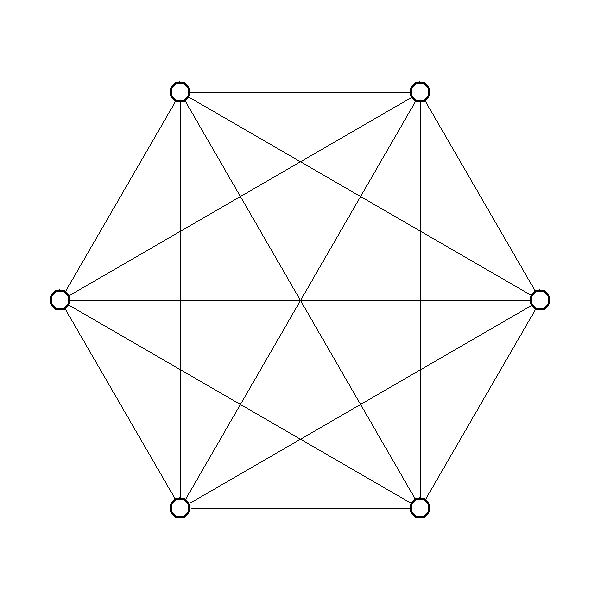
\includegraphics[scale = 0.19]{Pics/snek.png}
\end{figure}

\begin{exercise}
    Play the game and explore its properties.
    There are many connections between this game and Ramsey theory. (Side note: look up Ramsey Theory!)
\end{exercise}

\subsection{Miscellaneous Problems!}
\begin{exercise}
    In a game of tic-tac-toe, suppose that the first player plays in the corner, and the second player does NOT play in the center.
    Prove that the first player can force a win.
\end{exercise}

\begin{exercise}
In Determinant Tic-Tac-Toe, Player $1$ enters a $1$ into an empty $3\times 3$ matrix. Player $0$ counters with a $0$ in a vacant position, and play continues until the $3\times 3$ matrix is completed with five $1$'s and four $0$'s. Player $0$ wins if the determinant is $0$ and player $1$ wins otherwise. Assuming both players pursue optimal strategies, who wins and how?
\end{exercise}

\begin{exercise}
There are $n$ toothpicks in a row. The first player can take up to $n-1$ toothpicks. The second player can take at most the number of the toothpicks that the second has just taken. This continues until all the toothpicks are gone. The player who takes the last toothpick wins. For which $n$ does the first player have a winning strategy?
\end{exercise}

\begin{exercise}
Two players take turns naming positive integers that are not sums (with repetition) of previously named positive integers, with the player who names 1 being the loser. Prove that the game must end. Then prove that the first player can win.
\end{exercise}

\begin{exercise}
    Nine cards are on the table, numbered one through nine. The two players alternate picking up cards. The first player to have three cards summing to fifteen wins. If all cards are picked up without either player winning, the game is declared a ``draw''. Show that (i) if both players play perfectly, the game will be drawn, and (ii) if one player ``knows what's going on'', she can do very well, for example by starting with any of the even cards.
    % Hint: take a 3x3 magic square and keep track of the picked-up cards there. Notice that you are really playing some other more famous game.
\end{exercise}

\begin{exercise}
An integer $n$, unknown to you, has been randomly chosen in the interval $[1,2002]$ with uniform probability. Your objective is to select $n$ in an odd number of guesses. After each incorrect guess, you are informed whether $n$ is higher or lower, and you must guess an integer on your next turn among the numbers that are still feasibly correct. Show that you have a strategy so that the chance of winning exceeds $2/3$.
\end{exercise}

\begin{exercise}[Bachet's Game]
        Initially there are \(n>0\) checkers on the table.
        The legal moves consist of removing at least one but not more than \(k<n\) checkers from the table.
        The winner is the one to take the last checker.
        For what values of \(n\) will the first person have the winning strategy?
        How about the second person?
        What are the losing positions?
\end{exercise}

\emph{Hard!}

\begin{exercise}[1997 A2]
Players $1,2,3,\dots,n$ are seated around a table, and each has a single penny. Player $1$ passes a penny to Player $2$, who then passes two pennies to Player $3$. Player $3$ then passes one penny to Player $4$, who passes two pennies to Player $5$, and so on, players alternately passing one penny or two to the next player who still has some pennies. A player who runs out of pennies drops out of the game and leaves the table. Find an infinite set of numbers $n$ for which some player ends up with all $n$ pennies.
\end{exercise}

\begin{exercise}[1993 B2]
Consider the following game played with a deck of $2n$ cards, numbered from $1$ to $2n$. The deck is randomly shuffled and $n$ cards are dealt to each of the two players. Beginning with $A$, the player take turns discarding one of their remaining cards and announcing its number. The game ends as soon as the sum of the numbers on the discarded cards is divisible by $2n+1$. The last person to discard wins the game. Assuming optimal strategy by both $A$ and $B$, what is the probability that $A$ wins?
\end{exercise}

\begin{exercise}[2020 B2]
    Let \(k,n\in\ZZ\) with \(1\leq k<n\).
    Alice and Bob play a game with \(k\) pegs in a line of \(n\) holes.
    At the beginning of the game, the pegs occupy the \(k\) leftmost holes.
    A legal move consists of moving a single peg to any vacant hole that is further to the right.
    The players alternate moves, with Alice playing first.
    The game ends when the pegs are in the \(k\) rightmost holes, so whoever is next to play cannot move and therefore loses.
    For what values of \(n\) and \(k\) does Alice have a winning strategy?
\end{exercise}

\begin{exercise}[Warning: Topology!]
Let $Y$ be a non-empty topological space, $X$ a fixed subset of $Y$ and \(\mathcal{W}\) a family of subsets of $Y$ that have the following properties:
\begin{itemize}
    \item Each member of $\mathcal {W}$ has non-empty interior.
    \item Each non-empty open subset of $Y$ contains a member of $\mathcal {W}$. 
\end{itemize}
Players $P_{1}$ and $P_{2}$ alternately choose elements from $\mathcal {W}$ to form a sequence $W_{0}\supseteq W_{1}\supseteq \cdots W_{0}\supseteq W_{1}\supseteq \cdots$.
$P_{1}$ wins if and only if $X\cap \left(\bigcap _{n<\omega }W_{n}\right)\neq \emptyset$. 
Otherwise, $P_{2}$ wins.
This is called a general Banach-Mazur game, and you should try playing it (on a simple topological space of course)!

\end{exercise}

\end{document}